\chapter{Nederlandse Samenvatting}
\label{app:C}

\renewcommand{\figurename}{Figuur}

Online sociale netwerken nemen een steeds prominentere plaats in ons dagelijks leven als communicatienetwerk. Desondanks, bieden de door het Online Sociaal Netwerk (OSN) aangeboden privacy instellingen vaak onvoldoende bescherming voor de toevertrouwde data. Gebruikers kunnen opnieuw zelf bepalen wie er toegang krijgt tot hun data door cryptografische technieken toe te passen. 

In klassieke cryptografische systemen genereren gebruikers een private sleutel waarvan een publieke sleutel wordt afgeleid. De veiligheid van dergelijke systemen wordt gewaarborgd doordat het rekenkundig onhaalbaar is om in omgekeerde zin de private sleutel van de publieke sleutel af te leiden. Een publieke sleutel infrastructuur publiceert vervolgens de publieke sleutels van alle gebruikers. Bijgevolg kunnen gebruikers die nooit eerder communiceerden alsnog vertrouwelijke berichten uitwisselen door deze te encrypteren met elkaars publieke sleutel. Enkel de eigenaar van de private sleutel is vervolgens in staat om de berichten te decrypteren zodat de oorspronkelijke inhoud weer zichtbaar wordt.

Bestaande tools voor OSNs hebben echter moeite om algemeen aanvaard te worden bij gebruikers vanwege lage gebruiksvriendelijkheid en ingewikkeld beheer van cryptografische sleutels. Gebruikers kunnen immers moeilijk bewust kiezen wat geschikte sleutellengtes zijn of welke sleutels te vertrouwen zijn, zonder kennis van cryptografische primitieven.

In deze thesis, suggereren we een praktische oplossing die gebruik maakt van identiteitsgebaseerde encryptie om sleutelbeheer te vereenvoudigen en confidentialiteit op een OSN te waarborgen. Identiteitsgebaseerde encryptie laat immers toe om als publieke sleutel een herkenbare woordsequentie te nemen die de gebruiker uniek identificeert. Op die manier wordt meteen duidelijk wie de eigenaar is van de betreffende publieke sleutel waardoor complexe publieke sleutelinfrastructuren overbodig worden. 

Het nadeel van identiteitsgebaseerde encryptie is echter dat de private sleutel gegenereerd wordt door een publieke sleutel generator die bijgevolg volledig dient vertrouwd te worden. De publieke sleutel generator is immers in staat om \mbox{vertrouwelijke} berichten te decrypteren vermits hij de private sleutel van de ontvanger kent.

Door private sleutels op gedistribueerde wijze te genereren over verschillende publieke sleutel generatoren, bezit elke generator slechts een deel van de gebruikers' private sleutel. Samenwerkende publieke sleutel generatoren kunnen dan geen informatie afleiden over de private sleutels zolang hun aantal geen drempelwaarde $t$ overschrijdt. De confidentialiteit van de onderhandelde private sleutels wordt gegarandeerd zolang de verschillende generatoren geen motivatie hebben om samen te werken in deze architectuur.

\begin{figure}[ht]
    \begin{center}
    \scalebox{0.85}{
        \begin{tikzpicture}[auto, node distance=1mm,
            block/.style={rectangle,text width=6em,text centered,minimum height=11mm},
            line/.style={draw,very thick, ->},
            line2/.style={draw,very thick, <->},
            leg/.style={font=\scriptsize,text centered},
            ]
            % \draw[help lines] (-6,-5) grid (8,3);
            \draw[dashed] (-5,6) -- (5,6) -- (5,3) -- (-5,3) -- (-5,6);
            \path
                % title of PKG BOX
                (0, 6.5) node {\textbf{Verzameling van meerdere publieke sleutel generatoren}}
                
                % Bottom part
                (-5.5,0) node [block] (user) {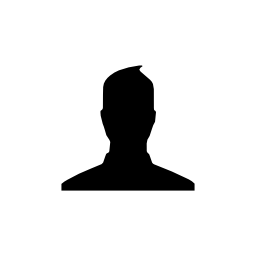
\includegraphics[scale=0.2]{img/fbuser.png}}
                (0,0) node [block] (fb) {
\includegraphics[scale=0.10]{img/fb_icon.png}}
                (5.5, 0) node [block] (friends) {
\includegraphics[scale=0.3]{img/fbfriends.png}}

                %Top part (PKG lists)
                (-3,4) node [block] (linkedin) {
\includegraphics[scale=0.1]{img/linkedin.png}}
                (-4,5) node [block] (fbpkg) {
\includegraphics[scale=0.06]{img/fb_icon.png}}
                (1.2,5) node [block] (gplus) {
\includegraphics[scale=0.08]{img/gplus.png}}
                (-2,5.2) node [block] (tumblr) {
\includegraphics[scale=0.1]{img/tumblr.png}}
                (2.8,4) node [block] (pin) {
\includegraphics[scale=0.05]{img/pinterest.png}}
                (4.2,5) node [block] (tor) {
\includegraphics[scale=0.1]{img/tor.png}}
                (-0.5,4) node [block] (twitter) {
\includegraphics[scale=0.05]{img/twitter.png}};

            \node[below=of fb] {\textbf{Facebook}};
            \node[below=of user] {\textbf{Gebruiker}};
            \node[below=of friends] (frdcaption) {\textbf{Deelverzameling van gewenste ontvangers}};
            \node[below=of frdcaption] {\textbf{zodat, $\mathcal{S}=\{\id{1},\id{2},\ldots,\id{\eta}\}$}};


            \begin{scope}[every path/.style=line]
                \path (user.east) -- (fb.west);               
            \end{scope}   

            % Legend
            \path (-2.8,0.35) node [leg] {Publiceer: $C\leftarrow$ Encrypteer($m$,$\mathcal{S}$)};
            \path (2.7,0.35) node [leg] {Download $C$};
            \node[right=of friends] {Decrypteer($C$)};
                
            \begin{scope}[every path/.style=line2]
                \path (fb) -- (friends);
                \path[dashed] (friends.north) -- (tor.south);
                \path[dashed] (5.1,1) -- (3.1,3.4);
                \path[dashed] (4.7,0.95) -- (0.5,3.5);
            \end{scope}
        \end{tikzpicture}
    }
    \end{center}
    \caption{Overzicht van een opstelling waarin meerdere OSNen een $(n,t)$-gedistribueerd publiek sleutel protocol aanbieden op basis van identiteitsgebaseerde encryptie. Een bericht $m$ wordt gepubliceerd op Facebook voor een deelverzameling $\mathcal{S}$ van ontvangers voor $t=3$. Het gedistribueerd sleutel protocol kan door elke organisatie ondersteund worden met een motivatie om de privacy op sociale netwerken te waarborgen.}
    \label{fig:overzicht}
\end{figure}

Figuur~\ref{fig:overzicht} toont een mogelijke opstelling in dewelke OSNen zelf de ondersteuning van de publieke sleutel generatoren verzorgen. Indien OSNen collectief hun gebruikersaantal zien dalen omwille van een slechte privacy policy, kan het een motivatie zijn om een dergelijke infrastructuur aan te bieden. Zeker in het kader van recente bekendmakingen van Edward Snowden over het spionageprogramma van de NSA, hebben OSNen elke motivatie om hun data te beschermen. Hoewel de OSNen bij een dergelijke opstelling geen gerichte reclame meer kunnen aanbieden, hebben ze er alle baat bij dat hun totaal gebruikersaantal niet verder afneemt. Doordat nooit meer dan $t$ rivaliserende OSN providers geneigd zijn om hun deel van de private sleutel bekend te maken, wordt de veiligheid van de opstelling gegarandeerd. Bemerk dat de publieke sleutel generatoren ook ondersteund kunnen worden door gesubsidieerde onderzoeksinstellingen of verschillende overheden.

Ge{\"i}nspireerd door het voorgaande, werken we aan de hand van identiteitsgebaseerde encryptie een algoritme uit dat toelaat om versleutelde informatie te delen met meerdere gebruikers zonder hun identiteit aan de buitenwereld te onthullen. De oplossing laat toe om versleutelde informatie te versturen aan gebruikers die nog niet expliciet hebben ingetekend om deel uit te maken van een dergelijke infrastructuur. Ten slotte, tonen we de haalbaarheid van onze oplossing aan door een open-source prototype te ontwikkelen dat praktisch bruikbaar is op Facebook en eenvoudig te veralgemenen valt naar andere bestaande OSNen.


%%% Local Variables: 
%%% mode: latex
%%% TeX-master: "thesis"
%%% End: 
